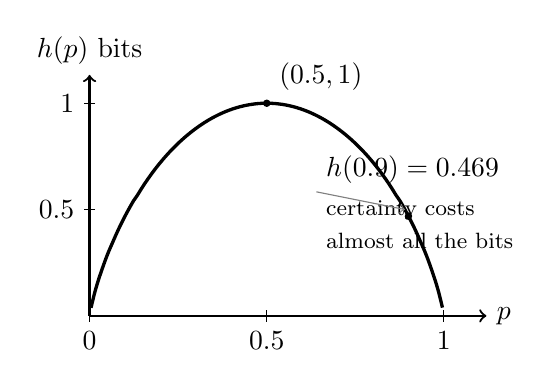
\begin{tikzpicture}[scale=0.9]
\draw[->, thick] (0,0) -- (5.6,0) node[right] {$p$};
\draw[->, thick] (0,0) -- (0,3.4) node[above] {$h(p)$ bits};
\foreach \x/\xl in {0/0, 2.5/0.5, 5/1}
  \draw (\x,0.08) -- (\x,-0.08) node[below] {\xl};
\foreach \y/\yl in {1.5/0.5, 3/1}
  \draw (0.08,\y) -- (-0.08,\y) node[left] {\yl};
% h(p) = -p log2 p - (1-p) log2(1-p), sampled
\draw[very thick, domain=0.02:4.98, smooth, samples=100]
  plot (\x, {3*(-(\x/5)*ln(\x/5)/ln(2) - (1-\x/5)*ln(1-\x/5)/ln(2))});
\fill (2.5,3) circle (1.5pt) node[above right=1pt] {$(0.5, 1)$};
\fill (4.5,{3*0.469}) circle (1.5pt);
\node[align=left, anchor=west] at (3.2,1.6) {$h(0.9)=0.469$\\[2pt]
  \footnotesize certainty costs\\ \footnotesize almost all the bits};
\draw[->, gray] (3.2,1.75) -- (4.45,1.5);
\end{tikzpicture}
